
%% bare_conf.tex
%% V1.4b
%% 2015/08/26
%% by Michael Shell
%% See:
%% http://www.michaelshell.org/
%% for current contact information.
%%
%% This is a skeleton file demonstrating the use of IEEEtran.cls
%% (requires IEEEtran.cls version 1.8b or later) with an IEEE
%% conference paper.
%%
%% Support sites:
%% http://www.michaelshell.org/tex/ieeetran/
%% http://www.ctan.org/pkg/ieeetran
%% and
%% http://www.ieee.org/

%%*************************************************************************
%% Legal Notice:
%% This code is offered as-is without any warranty either expressed or
%% implied; without even the implied warranty of MERCHANTABILITY or
%% FITNESS FOR A PARTICULAR PURPOSE! 
%% User assumes all risk.
%% In no event shall the IEEE or any contributor to this code be liable for
%% any damages or losses, including, but not limited to, incidental,
%% consequential, or any other damages, resulting from the use or misuse
%% of any information contained here.
%%
%% All comments are the opinions of their respective authors and are not
%% necessarily endorsed by the IEEE.
%%
%% This work is distributed under the LaTeX Project Public License (LPPL)
%% ( http://www.latex-project.org/ ) version 1.3, and may be freely used,
%% distributed and modified. A copy of the LPPL, version 1.3, is included
%% in the base LaTeX documentation of all distributions of LaTeX released
%% 2003/12/01 or later.
%% Retain all contribution notices and credits.
%% ** Modified files should be clearly indicated as such, including  **
%% ** renaming them and changing author support contact information. **
%%*************************************************************************


% *** Authors should verify (and, if needed, correct) their LaTeX system  ***
% *** with the testflow diagnostic prior to trusting their LaTeX platform ***
% *** with production work. The IEEE's font choices and paper sizes can   ***
% *** trigger bugs that do not appear when using other class files.       ***                          ***
% The testflow support page is at:
% http://www.michaelshell.org/tex/testflow/



\documentclass[conference]{IEEEtran}
% Some Computer Society conferences also require the compsoc mode option,
% but others use the standard conference format.
%
% If IEEEtran.cls has not been installed into the LaTeX system files,
% manually specify the path to it like:
% \documentclass[conference]{../sty/IEEEtran}





% Some very useful LaTeX packages include:
% (uncomment the ones you want to load)


% *** MISC UTILITY PACKAGES ***
%
%\usepackage{ifpdf}
% Heiko Oberdiek's ifpdf.sty is very useful if you need conditional
% compilation based on whether the output is pdf or dvi.
% usage:
% \ifpdf
%   % pdf code
% \else
%   % dvi code
% \fi
% The latest version of ifpdf.sty can be obtained from:
% http://www.ctan.org/pkg/ifpdf
% Also, note that IEEEtran.cls V1.7 and later provides a builtin
% \ifCLASSINFOpdf conditional that works the same way.
% When switching from latex to pdflatex and vice-versa, the compiler may
% have to be run twice to clear warning/error messages.






% *** CITATION PACKAGES ***
%
\usepackage{cite}
% cite.sty was written by Donald Arseneau
% V1.6 and later of IEEEtran pre-defines the format of the cite.sty package
% \cite{} output to follow that of the IEEE. Loading the cite package will
% result in citation numbers being automatically sorted and properly
% "compressed/ranged". e.g., [1], [9], [2], [7], [5], [6] without using
% cite.sty will become [1], [2], [5]--[7], [9] using cite.sty. cite.sty's
% \cite will automatically add leading space, if needed. Use cite.sty's
% noadjust option (cite.sty V3.8 and later) if you want to turn this off
% such as if a citation ever needs to be enclosed in parenthesis.
% cite.sty is already installed on most LaTeX systems. Be sure and use
% version 5.0 (2009-03-20) and later if using hyperref.sty.
% The latest version can be obtained at:
% http://www.ctan.org/pkg/cite
% The documentation is contained in the cite.sty file itself.








% *** MATH PACKAGES ***
%
%\usepackage{amsmath}
% A popular package from the American Mathematical Society that provides
% many useful and powerful commands for dealing with mathematics.
%
% Note that the amsmath package sets \interdisplaylinepenalty to 10000
% thus preventing page breaks from occurring within multiline equations. Use:
%\interdisplaylinepenalty=2500
% after loading amsmath to restore such page breaks as IEEEtran.cls normally
% does. amsmath.sty is already installed on most LaTeX systems. The latest
% version and documentation can be obtained at:
% http://www.ctan.org/pkg/amsmath





% *** SPECIALIZED LIST PACKAGES ***
%
%\usepackage{algorithmic}
% algorithmic.sty was written by Peter Williams and Rogerio Brito.
% This package provides an algorithmic environment fo describing algorithms.
% You can use the algorithmic environment in-text or within a figure
% environment to provide for a floating algorithm. Do NOT use the algorithm
% floating environment provided by algorithm.sty (by the same authors) or
% algorithm2e.sty (by Christophe Fiorio) as the IEEE does not use dedicated
% algorithm float types and packages that provide these will not provide
% correct IEEE style captions. The latest version and documentation of
% algorithmic.sty can be obtained at:
% http://www.ctan.org/pkg/algorithms
% Also of interest may be the (relatively newer and more customizable)
% algorithmicx.sty package by Szasz Janos:
% http://www.ctan.org/pkg/algorithmicx




% *** ALIGNMENT PACKAGES ***
%
%\usepackage{array}
% Frank Mittelbach's and David Carlisle's array.sty patches and improves
% the standard LaTeX2e array and tabular environments to provide better
% appearance and additional user controls. As the default LaTeX2e table
% generation code is lacking to the point of almost being broken with
% respect to the quality of the end results, all users are strongly
% advised to use an enhanced (at the very least that provided by array.sty)
% set of table tools. array.sty is already installed on most systems. The
% latest version and documentation can be obtained at:
% http://www.ctan.org/pkg/array


% IEEEtran contains the IEEEeqnarray family of commands that can be used to
% generate multiline equations as well as matrices, tables, etc., of high
% quality.




% *** SUBFIGURE PACKAGES ***
%\ifCLASSOPTIONcompsoc
%  \usepackage[caption=false,font=normalsize,labelfont=sf,textfont=sf]{subfig}
%\else
%  \usepackage[caption=false,font=footnotesize]{subfig}
%\fi
% subfig.sty, written by Steven Douglas Cochran, is the modern replacement
% for subfigure.sty, the latter of which is no longer maintained and is
% incompatible with some LaTeX packages including fixltx2e. However,
% subfig.sty requires and automatically loads Axel Sommerfeldt's caption.sty
% which will override IEEEtran.cls' handling of captions and this will result
% in non-IEEE style figure/table captions. To prevent this problem, be sure
% and invoke subfig.sty's "caption=false" package option (available since
% subfig.sty version 1.3, 2005/06/28) as this is will preserve IEEEtran.cls
% handling of captions.
% Note that the Computer Society format requires a larger sans serif font
% than the serif footnote size font used in traditional IEEE formatting
% and thus the need to invoke different subfig.sty package options depending
% on whether compsoc mode has been enabled.
%
% The latest version and documentation of subfig.sty can be obtained at:
% http://www.ctan.org/pkg/subfig




% *** FLOAT PACKAGES ***
%
%\usepackage{fixltx2e}
% fixltx2e, the successor to the earlier fix2col.sty, was written by
% Frank Mittelbach and David Carlisle. This package corrects a few problems
% in the LaTeX2e kernel, the most notable of which is that in current
% LaTeX2e releases, the ordering of single and double column floats is not
% guaranteed to be preserved. Thus, an unpatched LaTeX2e can allow a
% single column figure to be placed prior to an earlier double column
% figure.
% Be aware that LaTeX2e kernels dated 2015 and later have fixltx2e.sty's
% corrections already built into the system in which case a warning will
% be issued if an attempt is made to load fixltx2e.sty as it is no longer
% needed.
% The latest version and documentation can be found at:
% http://www.ctan.org/pkg/fixltx2e


%\usepackage{stfloats}
% stfloats.sty was written by Sigitas Tolusis. This package gives LaTeX2e
% the ability to do double column floats at the bottom of the page as well
% as the top. (e.g., "\begin{figure*}[!b]" is not normally possible in
% LaTeX2e). It also provides a command:
%\fnbelowfloat
% to enable the placement of footnotes below bottom floats (the standard
% LaTeX2e kernel puts them above bottom floats). This is an invasive package
% which rewrites many portions of the LaTeX2e float routines. It may not work
% with other packages that modify the LaTeX2e float routines. The latest
% version and documentation can be obtained at:
% http://www.ctan.org/pkg/stfloats
% Do not use the stfloats baselinefloat ability as the IEEE does not allow
% \baselineskip to stretch. Authors submitting work to the IEEE should note
% that the IEEE rarely uses double column equations and that authors should try
% to avoid such use. Do not be tempted to use the cuted.sty or midfloat.sty
% packages (also by Sigitas Tolusis) as the IEEE does not format its papers in
% such ways.
% Do not attempt to use stfloats with fixltx2e as they are incompatible.
% Instead, use Morten Hogholm'a dblfloatfix which combines the features
% of both fixltx2e and stfloats:
%
% \usepackage{dblfloatfix}
% The latest version can be found at:
% http://www.ctan.org/pkg/dblfloatfix

\usepackage{graphicx}
\usepackage{epstopdf}

% *** PDF, URL AND HYPERLINK PACKAGES ***
%
\usepackage{url}
% url.sty was written by Donald Arseneau. It provides better support for
% handling and breaking URLs. url.sty is already installed on most LaTeX
% systems. The latest version and documentation can be obtained at:
% http://www.ctan.org/pkg/url
% Basically, \url{my_url_here}.




% *** Do not adjust lengths that control margins, column widths, etc. ***
% *** Do not use packages that alter fonts (such as pslatex).         ***
% There should be no need to do such things with IEEEtran.cls V1.6 and later.
% (Unless specifically asked to do so by the journal or conference you plan
% to submit to, of course. )


% correct bad hyphenation here
\hyphenation{op-tical net-works semi-conduc-tor}


\begin{document}
%
% paper title
% Titles are generally capitalized except for words such as a, an, and, as,
% at, but, by, for, in, nor, of, on, or, the, to and up, which are usually
% not capitalized unless they are the first or last word of the title.
% Linebreaks \\ can be used within to get better formatting as desired.
% Do not put math or special symbols in the title.
\title{Security of Distribution Mechanisms for Linux and BSD Operating Systems}


% author names and affiliations
% use a multiple column layout for up to three different
% affiliations
\author{\IEEEauthorblockN{Gabriel Ewing}
\IEEEauthorblockA{Department of Electrical Engineering and\\Computer Science\\
Case Western Reserve University\\
Cleveland, Ohio}
\and
\IEEEauthorblockN{Kevin Nash}
\IEEEauthorblockA{Department of Electrical Engineering and\\Computer Science\\
Case Western Reserve University\\
Cleveland, Ohio}}

% conference papers do not typically use \thanks and this command
% is locked out in conference mode. If really needed, such as for
% the acknowledgment of grants, issue a \IEEEoverridecommandlockouts
% after \documentclass

% for over three affiliations, or if they all won't fit within the width
% of the page, use this alternative format:
% 
%\author{\IEEEauthorblockN{Michael Shell\IEEEauthorrefmark{1},
%Homer Simpson\IEEEauthorrefmark{2},
%James Kirk\IEEEauthorrefmark{3}, 
%Montgomery Scott\IEEEauthorrefmark{3} and
%Eldon Tyrell\IEEEauthorrefmark{4}}
%\IEEEauthorblockA{\IEEEauthorrefmark{1}School of Electrical and Computer Engineering\\
%Georgia Institute of Technology,
%Atlanta, Georgia 30332--0250\\ Email: see http://www.michaelshell.org/contact.html}
%\IEEEauthorblockA{\IEEEauthorrefmark{2}Twentieth Century Fox, Springfield, USA\\
%Email: homer@thesimpsons.com}
%\IEEEauthorblockA{\IEEEauthorrefmark{3}Starfleet Academy, San Francisco, California 96678-2391\\
%Telephone: (800) 555--1212, Fax: (888) 555--1212}
%\IEEEauthorblockA{\IEEEauthorrefmark{4}Tyrell Inc., 123 Replicant Street, Los Angeles, California 90210--4321}}




% use for special paper notices
%\IEEEspecialpapernotice{(Invited Paper)}




% make the title area
\maketitle

% As a general rule, do not put math, special symbols or citations
% in the abstract
\begin{abstract}
The abstract goes here.
\end{abstract}

% no keywords




% For peer review papers, you can put extra information on the cover
% page as needed:
% \ifCLASSOPTIONpeerreview
% \begin{center} \bfseries EDICS Category: 3-BBND \end{center}
% \fi
%
% For peerreview papers, this IEEEtran command inserts a page break and
% creates the second title. It will be ignored for other modes.
\IEEEpeerreviewmaketitle\


\section{Introduction}

An operating system is a piece of software that manages computer hardware resources
and provides a variety of services for computer programs.
The central core of an operating system, its kernel, is the first layer
above hardware itself. Due to of the depth of their functionality,
compromised operating systems can potentially yield a great deal more power
to an attacker than application software.\\
\indent Operating systems can be compromised by malicious computer software,
such as rootkits, in the course of normal operation. However, attacks can sometimes
be launched more easily against the distribution process itself. This can be done in such a way
that users unknowingly install a modified version of the expected operating
system. If successful, attacks that result in the distribution of a compromised
operating system can be both difficult to detect and
powerful.\\
\indent The open-source software model possesses a somewhat different attack surface that its closed- or shared-source counterparts.
Open-source operating systems often have much smaller core development teams
than popular commercial systems such as Windows and OS X. Open-source operating systems are rarely distributed using
physical media, which is the primary distribution mechanism for Windows.
The commercial interfaces that are requisite for online distribution of proprietary
software also have advantages and disadvantages in security that
are different from the security considerations that open-source distributors must account for.

\ldots\textit{Add more here}\ldots

\section{Operating System Distribution}

The specific process by which a new version of an operating system
travels from developer to end user differs between development teams.
Operating system developers establish their own schedule
standardizations, though the time between starting the release process
and the anticipated release typically takes no more than 90 days.
Teams may implement some steps less formally than others do,
though the general procedures are ubiquitous enough they can be
summarized by a few key steps.

\subsubsection{System Changes}

In an operating system's natural lifecycle, users tend to discover that
the system exhibits certain unexpected behaviors.
These bugs are reported, tracked, and hopefully fixed in code so that
users will not experience them in future versions of the operating system.
Users might request that entirely new features be added
or that existing, intentional behaviors be modified.
Even without user input, changes to the system inevitably
originate from within the development team; design paradigms change
and the world of security is ever-evolving.\\
\indent No matter the cause, an operating system's codebase can change
frequently. After enough changes are made to warrant a new release,
or at certain milestones in a predetermined development schedule,
developers stop making new changes in preparation for a code review.
The most developers of different operating systems will ``freeze''
or ``lock'' the code so that no more changes can be made.
Before the code freeze occurs, developers finish integrating their changes
and merge the development branch into a stable, or production, branch.
Of course, the naming of branches varies between projects.
Once the code is frozen, the interested public and, in almost all cases,
an internal body begin a code review.

\subsubsection{Code Review}

At this time, new features are tested for proper functionality,
and bug fixes are tested for robustness. In general, the code
is reviewed for proper practice and adherence to in-house standards.
A beta image is built and distributed to testers.
As necessary minor changes are made, such as those to update documentation,
fix remaining bugs, and address any discovered security issues,
additional beta images will be released for testing.

\subsection{Release Building}

Once the beta images are proven to meet quality standards,
a branch for the new version is created.
The most successful beta images will be included on the branch
as ``release candidates,'' a term for beta versions of software
that have the potential to be a finished product.

\begin{figure}[h!]
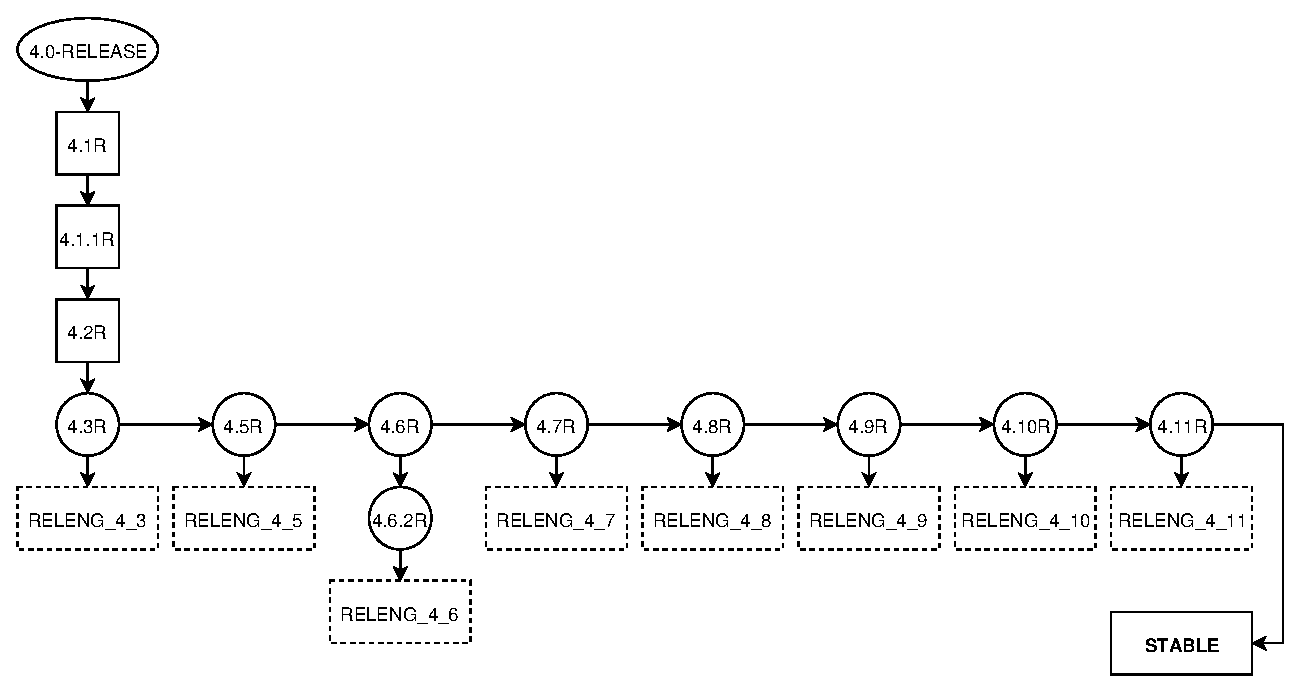
\includegraphics[width=\linewidth]{./images/FreeBSD_4.eps}
\caption{FreeBSD's RELENG\_4 (4.x STABLE Branch)}
\label{FreeBSD_4}
\end{figure}

\subsubsection{Pre-Distribution}

Body of text goes here\ldots

\subsection{Image Mirroring}

Body of text goes here\ldots

\subsubsection{Mirror Qualifications}

Body of text goes here\ldots

\subsubsection{Fetching Release}

Rsync, Zsync\ldots

\subsection{Distribution Methods}

Body of text goes here\ldots

\subsubsection{HTTP}

Body of text goes here\ldots

\subsubsection{FTP}

Body of text goes here\ldots

\subsubsection{BitTorrent}

Body of text goes here\ldots

\subsubsection{Physical Media}

Body of text goes here\ldots

\section{Attacks on Distribution}

Body of text goes here\ldots

\subsection{``Attack One''}

Body of text goes here\ldots

\subsubsection{Notable Usage}

Body of text goes here\ldots

\subsubsection{Countermeasures}

$N$ operating systems currently implement these countermeasures, including Foo, Bar, Baz\ldots

\textit{Visual aid goes here}

\subsection{``Attack Two''}

Body of text goes here\ldots

\subsubsection{Notable Usage}

Body of text goes here\ldots

\subsubsection{Countermeasures}

$N$ operating systems currently implement these countermeasures, including Foo, Bar, Baz\ldots

\textit{Visual aid goes here}

\subsection{Hash Collisions}
Providing a signed checksum is part of the best practices for securing download mechanisms. It allows the user to verify the authenticity of the checksum. Once the user is sure that the checksum is the one that they intended to download, they can use the same checksum algorithm to generate their own hash of the downloaded image. If the downloaded checksum and the generated checksum are identical, the user can then proceed, confident that the image they downloaded is the same one that the distribution maintainers published. However, certain commonly-used checksum algorithms are no longer strong enough to reliably verify the correctness of an image.\\
\indent Weak hashing algorithms introduce a vulnerability to the distribution process. Usually, an attacker that wishes to replace a published image also has to replace the associated published hash with the hash of the malicious image. Signed hashes alert users to this problem. If the hash of the malicious image is the same as the hash of the original image, though, the attacker does not need to replace the published hash and signing mechanisms are no longer sufficient.\\
\indent Hash collision attacks are particularly dangerous because normal protection policies do not detect their presence, allowing a malicious image to be installed silently. There are ways to detect a successful hash collision attack: one is that the malicious image would be different upon comparison to the original published image. Another is that distributed source code can be independently built and compared to the malicious image. If the distributed source code has also been replaced, then a code review or version control logs could offer clues. However, none of these checks is part of the standard practice recommended by an distribution that we surveyed. Because of this issue, weak checksum algorithms are a very dangerous practice.\\
\indent The MD5 hash algorithm was published in 1992 by Ronald Rivest~\cite{rivest1992md5}. Weaknesses in the algorithm were quickly discovered~\cite{md51993} and MD5 quickly dropped out of favor among the cryptographic hashing community. In 2004, a collision of the full MD5 algorithm was published~\cite{wang2004collisions}. MD5 collisions were used in proof-of-concept attacks on certificate authorities as early as 2005~\cite{md5attack}. While finding a collision that successfully installs and executes useful malicious tasks is more difficult than simply finding a collision, computing power has increased considerably since 2004 and it is not unreasonable to suspect that this capability exists in the world today.\\
\indent Unfortunately, many of the of the distributions that we surveyed, including Mint, Ubuntu, Debian, Arch, Slackware, and Mageia offer MD5 checksums. While none of them offer only MD5, many list it as the first option. MD5 is faster than the SHA variants, and is reliable in detecting random corruption from transmission, but the time to compute a checksum using a strong hash algorithm is still negligible compared to the time to download the image on any modern hardware. We consider offering MD5 checksums a poor practice because users with minimal cryptographic background may choose to only verify using MD5 and trust that a hashing algorithm used by the distribution is secure. Replacing an image and MD5 checksum would remain undetected until a stronger algorithm was tried and the distribution maintainers were notified.\\
\subsubsection{Countermeasures}
Distribution maintainers should remove MD5 checksums from their download pages and offer checksums generated by state-of-the-art algorithms. Additionally, they should compare the images offered by mirrors and their main download server to the image that they originally built on a regular basis. Users should verify downloaded images using the strongest algorithms available.
\section{External Risks}

Body of text goes here\ldots

\subsection{Re-Hosting and Ownership Hijacking}

Body of text goes here\ldots

\subsubsection{SourceForge}

SourceForge is a hosting service for open-source software. In 2015, the
website was accused of bundling malware with the binary project packages
that it offered for users to download. This caused some large projects to
abandon the site entirely~\cite{GIMPSourceForge}. While the company later
announced a change to this policy~\cite{SourceForgePolicy}, accusations
have continued~\cite{NmapSourceForge} and SourceForge can no longer be considered
a trustworthy hosting platform.\\
\indent Manjaro Linux was the sixth most-popular Linux distribution between March 2015
and March 2016 according to DistroWatch~\cite{DistroWatch}. According to our research,
SourceForge is the only download platform recommended and offered by
Manjaro. While downloads are available via torrent, the torrent
links are hosted by SourceForge as well and so the original seed may be of a compromised
image~\cite{ManjaroDownload}. We were unable to locate any alternative download mechanism.\\
\indent This means that there is a real possibility that as of this writing, image downloads
of Manjaro are bundled with malware. We recommend that users avoid downloading, installing
or running Manjaro Linux until the distribution maintainers review their practices and
provide alternatives for downloading.

\section{Best Consumer Practices}

\subsection{Choosing a Protocol}

Body of text goes here\ldots

\subsection{Verifying Mirrors}

Body of text goes here\ldots

\subsection{Building a Web of Trust}

Body of text goes here\ldots

\subsection{``Soft'' Risk Mitigation}

Sometimes it is best to rely on proven-stable releases. It can be harmful to be on the bleeding edge of development, although it is a service to the industry.

\section{Our Implementations}

Body of text goes here\ldots

% An example of a floating figure using the graphicx package.
% Note that \label must occur AFTER (or within) \caption.
% For figures, \caption should occur after the \includegraphics.
% Note that IEEEtran v1.7 and later has special internal code that
% is designed to preserve the operation of \label within \caption
% even when the captionsoff option is in effect. However, because
% of issues like this, it may be the safest practice to put all your
% \label just after \caption rather than within \caption{}.
%
% Reminder: the "draftcls" or "draftclsnofoot", not "draft", class
% option should be used if it is desired that the figures are to be
% displayed while in draft mode.
%
%\begin{figure}[!t]
%\centering
%\includegraphics[width=2.5in]{myfigure}
% where an .eps filename suffix will be assumed under latex, 
% and a .pdf suffix will be assumed for pdflatex; or what has been declared
% via \DeclareGraphicsExtensions.
%\caption{Simulation results for the network.}
%\label{fig_sim}
%\end{figure}

% Note that the IEEE typically puts floats only at the top, even when this
% results in a large percentage of a column being occupied by floats.


% An example of a double column floating figure using two subfigures.
% (The subfig.sty package must be loaded for this to work.)
% The subfigure \label commands are set within each subfloat command,
% and the \label for the overall figure must come after \caption.
% \hfil is used as a separator to get equal spacing.
% Watch out that the combined width of all the subfigures on a 
% line do not exceed the text width or a line break will occur.
%
%\begin{figure*}[!t]
%\centering
%\subfloat[Case I]{\includegraphics[width=2.5in]{box}%
%\label{fig_first_case}}
%\hfil
%\subfloat[Case II]{\includegraphics[width=2.5in]{box}%
%\label{fig_second_case}}
%\caption{Simulation results for the network.}
%\label{fig_sim}
%\end{figure*}
%
% Note that often IEEE papers with subfigures do not employ subfigure
% captions (using the optional argument to \subfloat[]), but instead will
% reference/describe all of them (a), (b), etc., within the main caption.
% Be aware that for subfig.sty to generate the (a), (b), etc., subfigure
% labels, the optional argument to \subfloat must be present. If a
% subcaption is not desired, just leave its contents blank,
% e.g., \subfloat[].


% An example of a floating table. Note that, for IEEE style tables, the
% \caption command should come BEFORE the table and, given that table
% captions serve much like titles, are usually capitalized except for words
% such as a, an, and, as, at, but, by, for, in, nor, of, on, or, the, to
% and up, which are usually not capitalized unless they are the first or
% last word of the caption. Table text will default to \footnotesize as
% the IEEE normally uses this smaller font for tables.
% The \label must come after \caption as always.
%
%\begin{table}[!t]
%% increase table row spacing, adjust to taste
%\renewcommand{\arraystretch}{1.3}
% if using array.sty, it might be a good idea to tweak the value of
% \extrarowheight as needed to properly center the text within the cells
%\caption{An Example of a Table}
%\label{table_example}
%\centering
%% Some packages, such as MDW tools, offer better commands for making tables
%% than the plain LaTeX2e tabular which is used here.
%\begin{tabular}{|c||c|}
%\hline
%One & Two\\
%\hline
%Three & Four\\
%\hline
%\end{tabular}
%\end{table}


% Note that the IEEE does not put floats in the very first column
% - or typically anywhere on the first page for that matter. Also,
% in-text middle ("here") positioning is typically not used, but it
% is allowed and encouraged for Computer Society conferences (but
% not Computer Society journals). Most IEEE journals/conferences use
% top floats exclusively. 
% Note that, LaTeX2e, unlike IEEE journals/conferences, places
% footnotes above bottom floats. This can be corrected via the
% \fnbelowfloat command of the stfloats package.




\section{Conclusion}
The conclusion goes here.




% conference papers do not normally have an appendix


% use section* for acknowledgment
% trigger a \newpage just before the given reference
% number - used to balance the columns on the last page
% adjust value as needed - may need to be readjusted if
% the document is modified later
%\IEEEtriggeratref{8}
% The "triggered" command can be changed if desired:
%\IEEEtriggercmd{\enlargethispage{-5in}}

% references section

% can use a bibliography generated by BibTeX as a .bbl file
% BibTeX documentation can be easily obtained at:
% http://mirror.ctan.org/biblio/bibtex/contrib/doc/
% The IEEEtran BibTeX style support page is at:
% http://www.michaelshell.org/tex/ieeetran/bibtex/
\bibliography{references.bib}
\bibliographystyle{IEEEtran}
% argument is your BibTeX string definitions and bibliography database(s)
%\bibliography{IEEEabrv,../bib/paper}
%
% <OR> manually copy in the resultant .bbl file
% set second argument of \begin to the number of references
% (used to reserve space for the reference number labels box)
%\newcommand{\bibspace}[1] {\hskip 0.5em}
%\begin{thebibliography}{1}
%\end{thebibliography}

% that's all folks
\end{document}
